\documentclass{article}
% Damit die Verwendung der deutschen Sprache nicht ganz so umst\"andlich wird,
% sollte man die folgenden Pakete einbinden: 
\usepackage[latin1]{inputenc}% erm\"oglich die direkte Eingabe der Umlaute 
\usepackage[T1]{fontenc} % das Trennen der Umlaute
% \usepackage{ngerman} % hiermit werden deutsche Bezeichnungen genutzt und 
                     % die W\"orter werden anhand der neue Rechtschreibung 
		     % automatisch getrennt.
\usepackage{authblk}
\usepackage{hyperref}
\usepackage{cleveref}
\usepackage{graphicx}

\title{Reinforcement Learning Exercise 1}
\author{Alexander J\"aggle}
\author{Johannes Haberstock}
\author{Daniel Arnold}

\affil{M.Sc. Autonomous Systems, University of Stuttgart}

\date{\today}
% Hinweis: \title{um was auch immer es geht}, \author{wer es auch immer 
% geschrieben hat} und  \date{wann auch immer das war} k\"onnen vor 
% oder nach dem  Kommando \begin{document} stehen 
% Aber der \maketitle Befehl mu\ss{} nach dem \begin{document} Kommando stehen! 
\begin{document}

\maketitle

\section{Multi-armed Bandits}

\begin{itemize}
    \item[a)] The probability of the greedy action being selected is $p = .5$ since $p = 1- \epsilon$.   
    \item[b)] {
    \begin{itemize}
        \item[1.] random = [{1,2,5}]
        \item[2.] greedy = [{3,4}]
    \end{itemize}
    }
\end{itemize}


\paragraph{Explanation to b)}
Before step three is executed, only the rewards for action $1$ and action $2$ are known, which both are 1. 
Every other action, which was not explored yet, is assumed with a reward of 0. Thus, at timestep $t = 3$, 
action $2$ with a reward of 1 was selected at greedy. 

A similar scenario happened at timestep $t = 4$, when action-value estimates $Q$ are known. For timestep $t = 3$,
the action-value estimate is 1.5, while the other two estimates are 1 respectively 0. Since the next action, which
was selected was action $2$, and thus it was greedy. 

\section{Action Selection Strategies}
The solution of our group will be submitted as \textit{ex01-bandits.py} and is also available on our 
\href{https://github.com/DesmoAlex/ReinforcementLearning_UniStgt/tree/master/ex01-bandits}{GitHub}.

\begin{itemize}
    \item[a)] Changes were made between line 24 - 54 
    \item[b)] Changes were made between line 58 - 99
    \item[c)] E-Greedy performs better with a total amount of 805.76 compared to a score of 797.63
                of the Greedy as can be seen in \cref{fig:comparison}. After roughly 300 executions, e-greedy surpasses the greedy in amount of
                rewards.   
                \item[d)] Possible ways to improve the methods is to change $\epsilon$ or increase the number of executions.
\end{itemize}
            
\begin{figure}[h]
    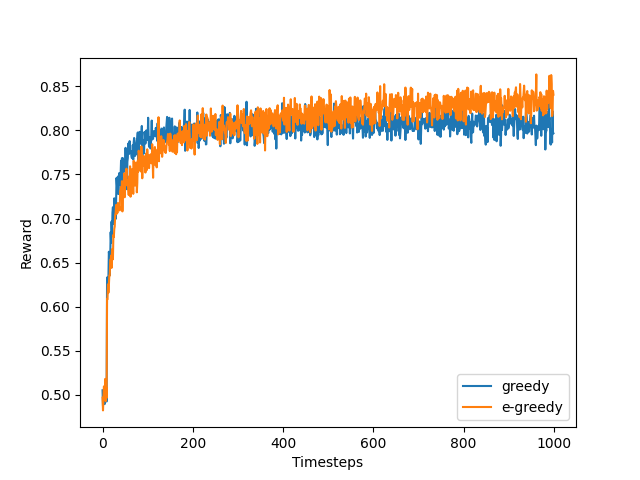
\includegraphics[scale=0.8]{Figure_1.png}
    \caption{$\epsilon$-Greedy vs. Greedy}
    \label{fig:comparison}
\end{figure}

\end{document}